\section{Object definitions and Event selection}

\subsection{Event cleanup and vertex selection}

Events with at least one primary vertex passing an OR combination
of the HLTs shown on table \ref{tab:HLTDatasets}, and containing at least three
leptons (number of muons and electrons) are selected provided that its
missing energy $E_T^{Miss}$ is greater than $40~GeV$.

In addition, the following flags are required for the event:

\begin{itemize}
  \item \verb|Flag_goodVertices|
  \item \verb|Flag_globalSuperTightHalo2016Filter|
  \item \verb|Flag_HBHENoiseFilter|
  \item \verb|Flag_HBHENoiseIsoFilter|
  \item \verb|Flag_EcalDeadCellTriggerPrimitiveFilter|
  \item \verb|Flag_BadPFMuonFilter|
\end{itemize}

One additional flag is required for the year 2017, 2018:

\begin{itemize}
\item \verb|Flag_ecalBadCalibFilterV2|
\end{itemize}

Events are then splitted in four channels depending on the leptonic flavour of the
diboson decay:

\begin{description}
\item[$\bullet$3e] three electrons and missing transverse energy are found, two of the
  electrons correspond to the decay of the $Z$ boson and the remaining electron corresponds
  to the decay of the $W$ boson. $Z\rightarrow e^{+}e^{-} W\rightarrow e+\nu$
  The three electrons are expected to leave traces on the
  tracker subsystem with low curvature due to their high transverse momentum and
  energy depositions are expected in the electromagnetic calorimeter
  The signature left on the CMS detector is shown on figure \ref{fig:Fireworks_eeev}.
\item[$\bullet$2e+1mu] two electrons, one muon and missing transverse energy are found,
  the two electrons correspond to the decay of the $Z$ boson and the muon corresponds to the
  decay of the $W$ boson. $Z\rightarrow e^{+}e^{-} W\rightarrow \mu+\nu$ the two electrons are
  expected to leave traces on the tracker subsystem with low curvature and energy
  depositions are expected in the electromagnetic calorimeter while the muon leaves
  traces in the tracker and muon subsytem. The signature left on the CMS
  detector is shown on figure \ref{fig:Fireworks_eemuv}.
\item[$\bullet$2mu+1e] two muons, one electron and missing transverse energy are found,
  the two muons correspond to the decay of the $Z$ boson and the electron corresponds to the
  decay of the $W$ boson. $Z\rightarrow \mu^{+}\mu^{-} W\rightarrow e+\nu$ the two
  muons leave traces on the tracker and muon subsystems with negligible curvature due
  to its high transverse momentum while the electron is expected to leave hits in
  the tracker and energy deposition in the electromagnetica calorimeter.
  The signature left on the CMS detector is shown on figure \ref{fig:Fireworks_mumuev}.
\item[$\bullet$3mu] three muons and missing transverse energy are found, the muon pair
  correspond to the decay of the $Z$ boson and the remianing muon corresponds
  to the decay of the $W$ boson. $Z\rightarrow \mu^{+}\mu^{-} W\rightarrow \mu+\nu$.
  The three muons are expected to leave traces on the tracker subsystem and muon chambers
  with low curvature due to their high transverse momenta. The signature
  left on the CMS detector is shown on figure \ref{fig:Fireworks_eemuv}.
\end{description}

\begin{figure}
  \centering
  \subfigure[Projection on the $\rho-\phi$ plane. \label{fig:A_RhoPhi}]{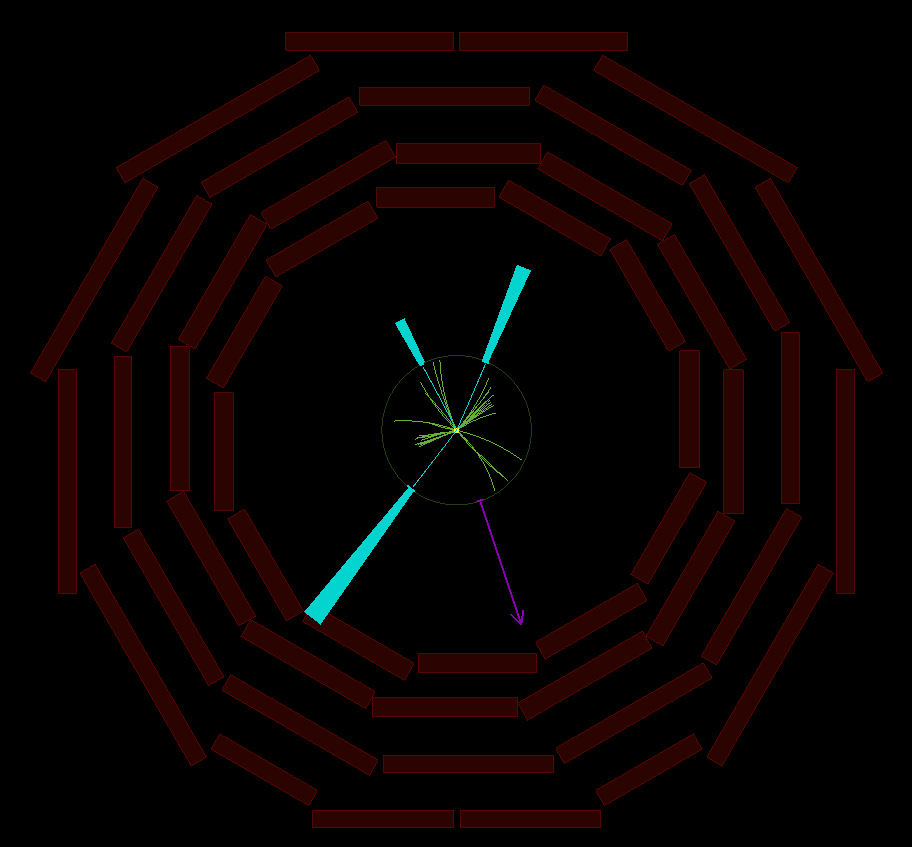
\includegraphics[width=0.8\linewidth]{fig/Fireworks/A_RhoPhi.png}}
  \vfil
  \subfigure[Projection on the $\rho-z$ plane\label{fig:A_RhoZ}]{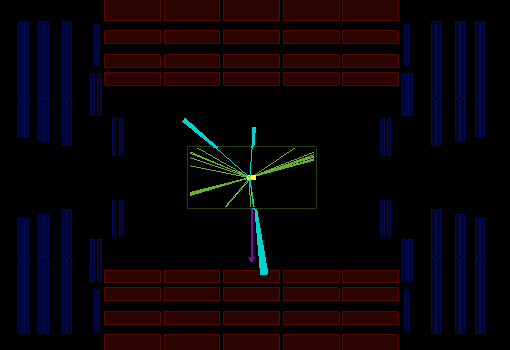
\includegraphics[width=0.40\linewidth]{fig/Fireworks/A_RhoZ.png}}
  \subfigure[3D view\label{fig:A_Rho3D}]{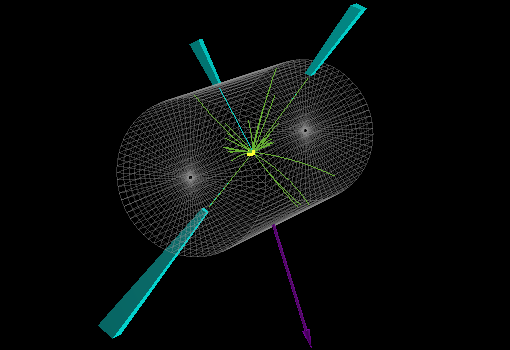
\includegraphics[width=0.40\linewidth]{fig/Fireworks/A_3D.png}}
  \caption{Example of the signature left on the detector by a signal-like event
    for the $eee\nu$ channel. This event was taken on July 13th 2018. Run: $319579$,
    Lumiblock: $2957$, Event: $4487890911$. The reconstructed primary vertex is shown in yellow.
    Depositions on the electromagnetic calorimeter and tracks left by the three electrons
    are shown in turquoise, the negligible curvature
    shown by their tracks is a reflection of their high transverse momentum.
    The amount of missing transverse energy is proportional to the length of the purple arrow. Low momentum
    tracks for particle-flow candidates in the inner tracker are shown in green for
    reference, these PF candidates are filtered by the preselection. }
  \label{fig:Fireworks_eeev}
\end{figure}


\begin{figure}
  \centering
  \subfigure[Projection on the $\rho-\phi$ plane. \label{fig:B_RhoPhi}]{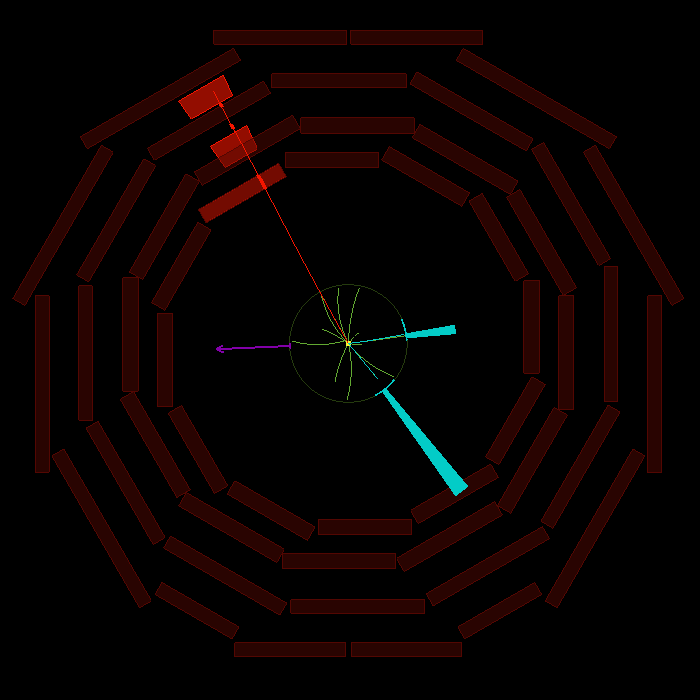
\includegraphics[width=0.8\linewidth]{fig/Fireworks/B_RhoPhi.png}}
  \vfil
  \subfigure[Projection on the $\rho-z$ plane\label{fig:B_RhoZ}]{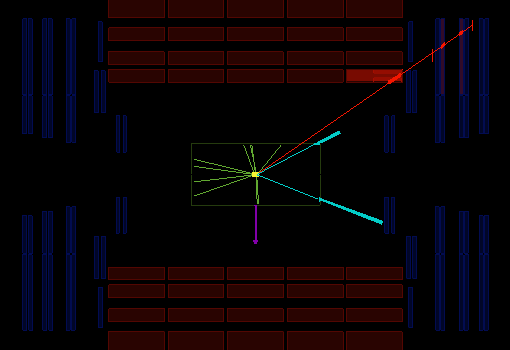
\includegraphics[width=0.40\linewidth]{fig/Fireworks/B_RhoZ.png}}
  \subfigure[3D view\label{fig:B_Rho3D}]{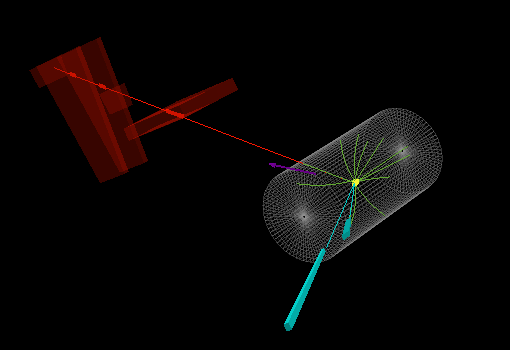
\includegraphics[width=0.40\linewidth]{fig/Fireworks/B_3D.png}}
  \caption{Example of the signature left on the detector by a signal-like event
    for the $ee\mu\nu$ channel. This event was taken on October 21st 2018. Run: $32500$,
    Lumiblock: $188$, Event: $346288517$. The reconstructed primary vertex is shown in yellow.
    Depositions on the electromagnetic calorimeter
    and tracks left by the electronic pair are shown in turquoise, the negligible curvature
    shown by their tracks is a reflection of their high transverse momentum. Tracks left by the muon
    in the tracker detector and muon chambers are shown in red, in this particular event it
    is possible to see the muon will be classified as a global-High Pt muon as its traces
    are found in the tracker system and beyond the first station of the muon subsystem.
    The amount of missing
    transverse energy is proportional to the length of the purple arrow. Low momentum
    tracks for particle-flow candidates in the inner tracker are shown in green for
    reference, these PF candidates are filtered by the preselection. }
  \label{fig:Fireworks_eemuv}
\end{figure}

\begin{figure}
  \centering
  \subfigure[Projection on the $\rho-\phi$ plane. \label{fig:C_RhoPhi}]{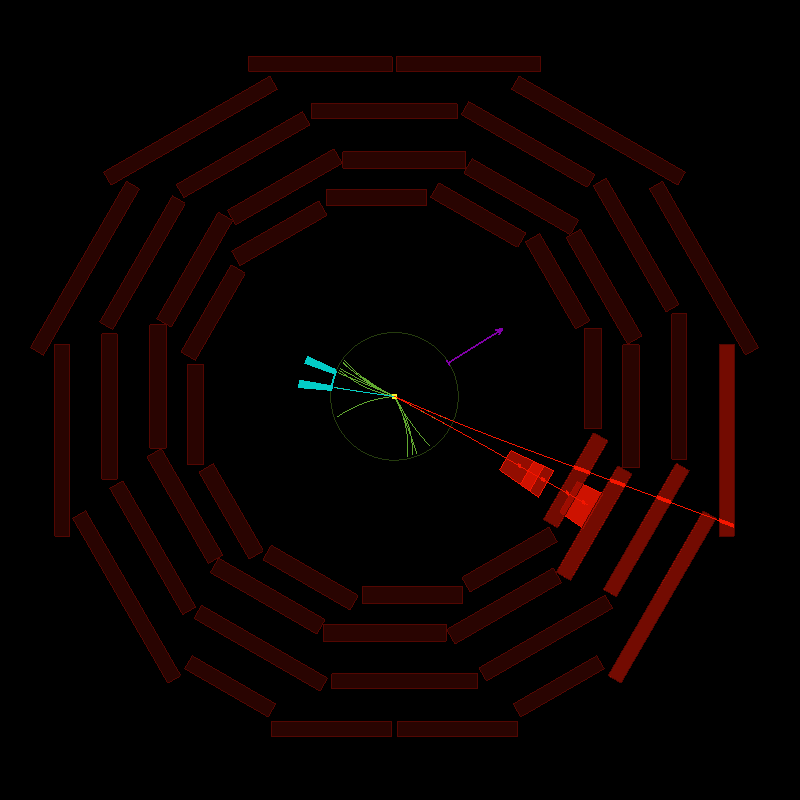
\includegraphics[width=0.8\linewidth]{fig/Fireworks/C_RhoPhi.png}}
  \vfil
  \subfigure[Projection on the $\rho-z$ plane\label{fig:C_RhoZ}]{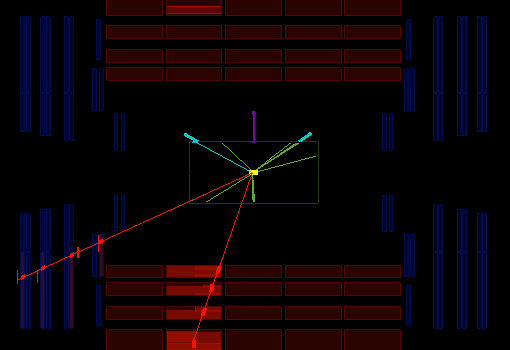
\includegraphics[width=0.40\linewidth]{fig/Fireworks/C_RhoZ.png}}
  \subfigure[3D view\label{fig:C_Rho3D}]{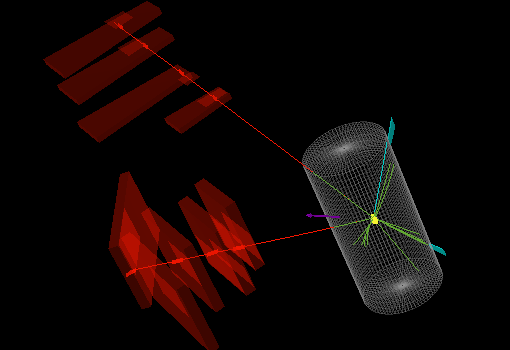
\includegraphics[width=0.40\linewidth]{fig/Fireworks/C_3D.png}}
  \caption{Example of the signature left on the detector by a signal-like event
    for the $\mu\mu e \nu$ channel. This event was taken on August 14th 2018.
    Run: $321295$, Lumiblock: $553$, Event: $873839127$. The reconstructed primary vertex is shown in yellow.
    The deposition on the electromagnetic calorimeter and tracks left by the electron are shown in turquoise,
    the negligible curvature shown by their tracks is a reflection of their high transverse momentum.
    Tracks left by the muon pair in the tracker detector and muon chambers are shown in red, it
    is possible to see the muon will be classified as a global-High Pt muon as their traces
    are found in the tracker system and beyond the first station of the muon subsystem.
    The amount of missing
    transverse energy is proportional to the length of the purple arrow. Low momentum
    tracks for particle-flow candidates in the inner tracker are shown in green for
    reference, these PF candidates are filtered by the preselection. }
  \label{fig:Fireworks_mumuev}
\end{figure}

\begin{figure}
  \centering
  \subfigure[Projection on the $\rho-\phi$ plane. \label{fig:D_RhoPhi}]{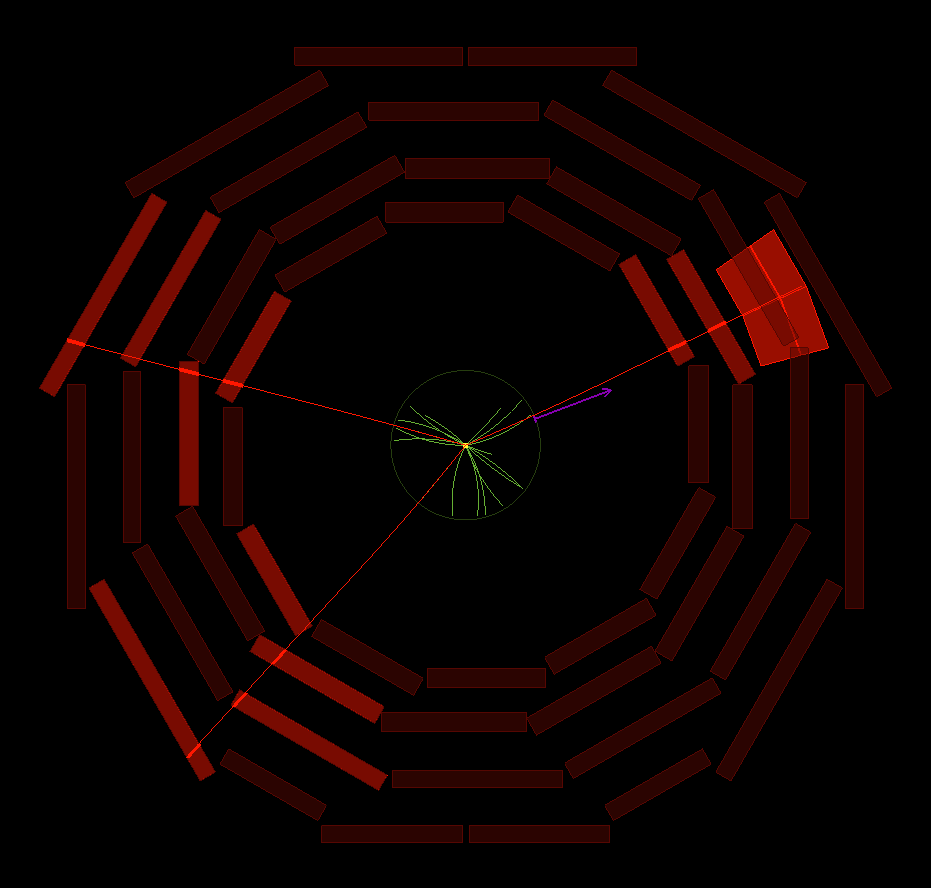
\includegraphics[width=0.8\linewidth]{fig/Fireworks/D_RhoPhi.png}}
  \vfil
  \subfigure[Projection on the $\rho-z$ plane\label{fig:D_RhoZ}]{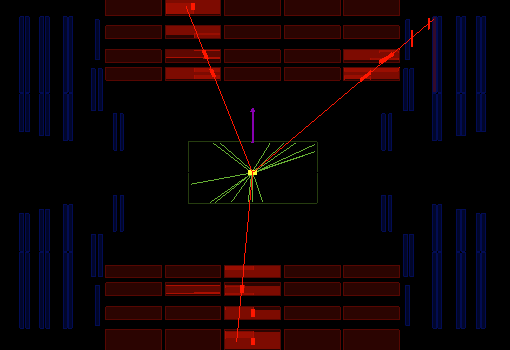
\includegraphics[width=0.40\linewidth]{fig/Fireworks/D_RhoZ.png}}
  \subfigure[3D view\label{fig:D_Rho3D}]{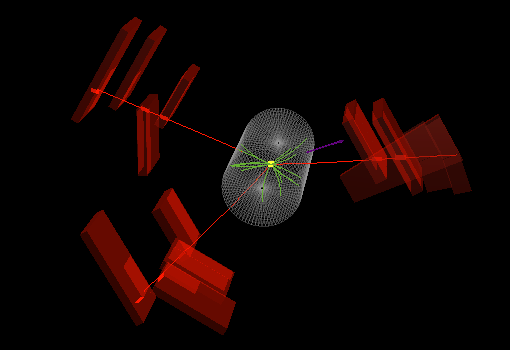
\includegraphics[width=0.40\linewidth]{fig/Fireworks/D_3D.png}}
  \caption{Example of the signature left on the detector by a signal-like event
    for the $\mu\mu\mu\nu$ channel. This event was taken on July 21st 2018.
    Run: $320024$, Lumiblock: $211$, Event: $355149645$. The reconstructed primary vertex is shown in yellow.
    Tracks left by the muon pair in the tracker detector and muon chambers are shown in red,
    the negligible curvature shown by their tracks is a reflection of their high transverse momentum.
    it is possible to see the muon will be classified as a global-High Pt muon as their traces
    are found in the tracker system and beyond the first station of the muon subsystem.
    The amount of missing
    transverse energy is proportional to the length of the purple arrow. Low momentum
    tracks for particle-flow candidates in the inner tracker are shown in green for
    reference, these PF candidates are filtered by the preselection. }
  \label{fig:Fireworks_mumumuv}
\end{figure}






\subsection{High Level Trigger Selection}

The table \ref{tab:HLTDatasets} shows the HLTs used and the different datasets used for the three years.
Each event is required to pass either the Muon or Electron triggers based on the high-Pt
recommendations from the POG.

Due to the presence of multiple leptonic flavors in the final state, we require
the signal events to satisfy at least one of the following High Level Trigger
Requirements.

We reproduce the High Level Trigger requirements by applying the corresponding
$p_T$ threshold



\begin{table}[h]
\centering
\caption{List of HLT requirements and its associated dataset.}
\begin{tabular}{|l|l|l|}
\hline
Year & Dataset & HLT                \\ \hline
2016 & SingleMuon     & HLT\_TkMu50 \\
     &                & HLT\_Mu50   \\
     & SingleElectron & HLT\_Ele27\_WPTight\_Gsf  \\
     & SinglePhoton   & HLT\_Photon175            \\ \hline
2017 & SingleMuon     & HLT\_Mu50       \\
     &                & HLT\_OldMu100   \\
     &                & HLT\_TkMu100    \\
     & SingleElectron & HLT\_Ele35\_WPTight\_Gsf  \\
     & SinglePhoton   & HLT\_Photon200            \\ \hline
2018 & SingleMuon & HLT\_Mu50     \\
     &            & HLT\_OldMu100 \\
     &            & HLT\_TkMu100  \\ \hline
     & EGamma     & HLT\_Ele32\_WPTight\_Gsf \\
     &            & HLT\_Photon200           \\ \hline
\end{tabular}
\label{tab:HLTDatasets}
\end{table}


\subsection{Lepton Selection}

\subsection{Electron Selection}

\verb|Electron| collection in \verb|NanoAOD|

Electrons are reconstructed from hits in the different
layers of the tracker and energy deposits in the scintillating crystalls
across the $\eta-\phi$ plane in the Electromagnetic Calorimeter.

The electron's sign charge can be identified by its signature in the tracker
due to the presence of the strong magnetic field in the CMS detector.

Electrons in this analysis are required to be within the ECAL fiducial
region i.e $\abs{eta}<2.5$ excluding the transition region betwen the
barrel and the endcaps $1.4442<\abs{eta}<1.5660$.

Electron identification is based on a cut based ID as defined by the
EGamma POG. Depending on the channel, this requirement
may ask for \emph{loose} or \emph{tight} electrons, the former with an
average efficiency of approximately 95\% and 70\% for
the latter ~\cite{EGammaPOG_el}.

\subsection{Muon Selection}

\verb|Muon| collection in \verb|NanoAOD|

The muon objects in this analysis can be divided into two categories:
Tracker and highPt Global muons ~\cite{MuonPOG}.

Muons are required to be within the pseudorapidity range $\abs{eta}<2.4$ and
to have a minimum transverse momentum of $P_t=20$. Additionally the leading muon of
the event is required to have $P_t>52$ in line with the trigger plateau.

Transverse momentum is measured with the TuneP algorithm

\subsection{Missing Transverse Energy}

The missing transverse energy $E_T$ is reconstructed with the particle flow
algorithm ~\cite{particleflow}

\subsection{Z Candidate}

Two same flavored, opposite charged leptons are required to reconstruct a Z
candidate. If more than one pair is found, the one with reconstructed mass
closer to the nominal mass $M_z= 91.1876 GeV$ is chosen. The pair's mass
is required to fall in the Z mass window $ 70. GeV < M_Z < 111.$. In favor of an
increase in the signal efficiency the opposite charged requirement is dropped
for the $3e0\mu$ category.

If the Z candidate is formed from a muon pair with a leading (subleading) muon with
a transverse momentum of at least $P_t=70 GeV$ ($P_t=10GeV$). One of the
muons is required to pass two additional requirements: being a global high-Pt muon and a
particle-flow candidate. In the case of electrons, the requirement is to pass the
selection criteria of the cut-based \emph{loose} ID and a transverse momentum of
at least $P_t=27GeV$ (2016) matching the trigger plateau, $P_t=35GeV$ (2017),
$P_t=32GeV$ (2018).

The event is rejected if the distance in the $\eta-\phi$ plane for the two
leptons product of the decay of the Z is less than $1.5$.

\subsection{W Candidate}

The neutrino coming from The $W \rightarrow l\nu$ candidate escapes undetected,
and therefore the following assumptions are made in order to perform a kinematic
reconstruction of the $W$ candidate: there is no additional sources of missing
energy, and consequently $E_{Pt}^{miss}$ is considered the transverse momentum
corresponding to the undetected neutrino. The longitudinal momentum $P_z$ can be
recovered by imposing the $M_W = 80.379 GeV $ nominal mass and $M_\nu = 0.$

As $\eta$ is unknown for the Missing Energy transverse, the neutrino 4-vector is
not well defined. However, by assuming the mass of W[pdg] the longitudinal component
of the neutrino is reduced to a quadratic equation. The less energetic of the
solutions gives the correct value ~70\% of the time according to simulation [AN].
When no real solutions are available (transverse mass > W Mass), the invariant
mass is set to the reconstructed transverse mass and we are left with two real
identical solutions. The transverse mass may be higher to W mass due to detector
resolution effects.

$W$ boson is reconstructed from the remaining lepton and the missing energy
$E_T^{miss}$. The ramining lepton is required to be either
a \emph{tight} electron or a global High-Pt muon with a transverse momentum
of at least $Pt=50GeV$.

\subsection{WZ Candidate}

* Mass of the three leptons system should be greater than $120GeV$
* The sum of the transverse momentum of the leptons should be greater than $110GeV$


\subsection{Lepton Misidentification}

